\chapter{Introduction}
\label{sec:intro}

\section{Motivation}
A sequenced route query is defined as finding the shortest path from a starting point towards a possible destination, passing through multiple locations, defined by their category type. There has been significant research and proposed approaches on the topic, but there is not a developed query language to answer this types of queries. The work in this thesis has been focused on researching the topic of sequenced route queries and designing a language to enable the user to express his need in the form of a user query in a flexible manner, such as applying different constraints on the route to be found.

\textbf{Example:}
Suppose that a user is planning a trip to town: he first wants to go to a restaurant for lunch, then he wants to stop by a bank, then he meets a friend in the shopping mall and after that he plans to have a dinner at a restaurant. In this specific scenario, the user wants to express his wish for the restaurant to be the same, because he may prefer a route where the equality of the two restaurant PoIs is more important to him than the length of the route.

With existing approaches, the user may get the shortest route \cite{OSR} or all routes that satisfy the semantic similarity and length conditions equally \cite{semanticSRQ}, but that does not guarantee the equality of the two restaurant PoIs. Also finding k optimal routes answering the user's SRQ and then filtering out the routes where the two PoIs of type restaurant are equal has proven to not always generate a result, which is why in this thesis an optimal approach is presented.

Specific constrains such as the equality in the given example above are proposed in the thesis as operators on the query. Existing approaches have been used to transform the complex user query and changes to the approaches have been made in order to retrieve a desired result. 

\section{Problem definition}
We have a starting point $sp$ and a category sequence $M = (c_1, c_2, ..., c_n)$, which constitutes the query, defined by the user. The constraints for this query can be applied as operators.
For this query a route $(r_1, r_2, ..., r_n)$, defined as a sequence of PoIs, is calculated. \newline

\textbf{Graph model:}
The graph is constructed using Berlin's spatial datasets from \cite{datasets}, structured in separate CSV files for the crossroads, roads and points of interest.

For the implementation of the operators the datasets are imported into a graph structure of nodes and edges, where each node has a unique id, its latitude and longitude and a list of PoIs that have been mapped to it and each edge has a source and destination node and the distance between the two nodes in kilometers as parameters. Each PoI is mapped to the nearest crossroad and has a unique id, a type, its latitude and longitude and the distance to the node it is mapped to. \newline

% Not used anymore
\iffalse
The graph is constructed using the Neo4j graph database as seen in \ref{fig:neo4jmodel}
The crossroads are defined as nodes, labeled CROSSROAD, with attributes id, longitute and latitude, the roads are mapped as relationships, labeled ROAD, with attribute distance. A PoI is mapped to the nearest CROSSROAD, using a relationship HAS-POI, with attributes id and a list of possible category types it belongs to. \cite{evagian}

\begin{figure}[h]
	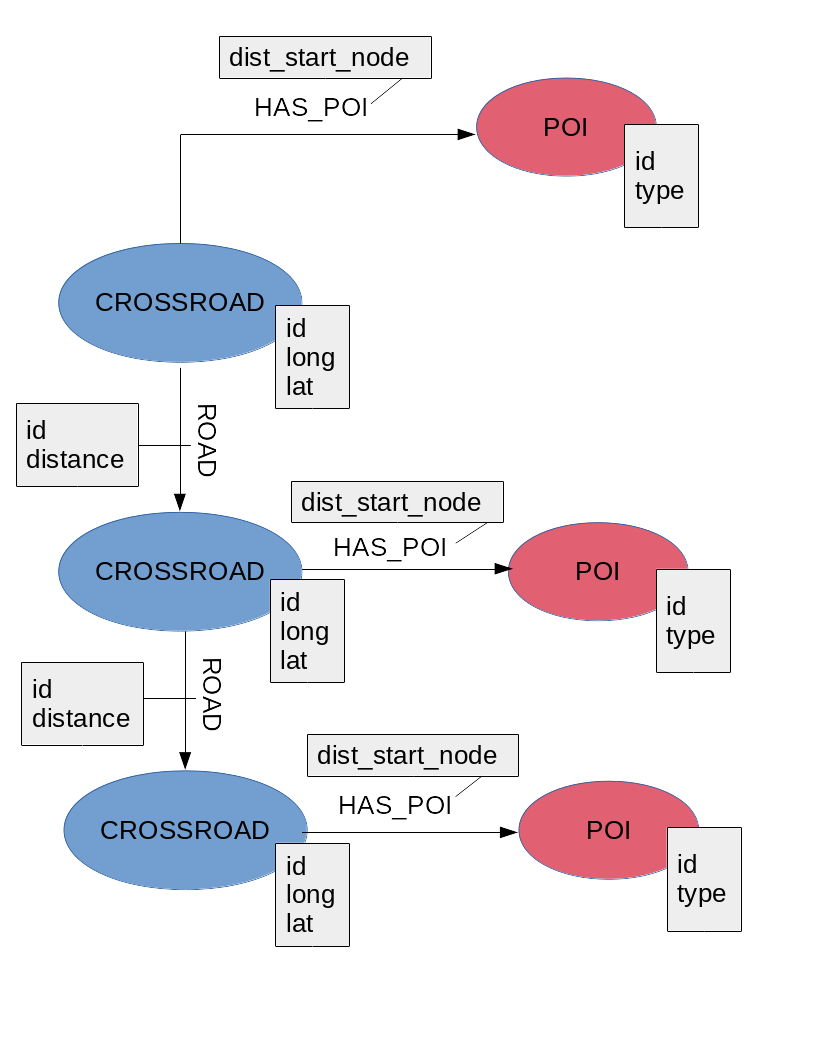
\includegraphics[scale=0.4]{images/Neo4j-model.png}
	\centering
	\caption{Neo4j Model\cite{evagian}}
	\label{fig:neo4jmodel}
\end{figure}
\fi

 
The map used for implementation and testing is the road network of Berlin, with 428769 crossroads, 504229 roads, 5548 PoIs and 7 category types: restaurant (2081), coffee shop (1002), atms/banks (597), movie theaters (141), pharmacies (589), pubs/bars (958), gas stations (180). 
\newline

% ???
\section{Challenges}
\todo[color=yellow!40]{Challenges}

% ???
% Shortly presenting the algorithms for the operators
\section{Contributions}
\todo[color=yellow!40]{Contributions}

The remainder of the thesis is organized as follows: First I review the related work that has been done on the topic of SRQ in Section 2. In Section 3 I cover the proposed operators and go into details on some of them in three separate sections for each of them: Design, Implementation and Evaluation. Finally, I conclude the thesis by summing up the progress made on the subject and discuss future work.